\documentclass[12pt]{article}
\usepackage[margin=1in]{geometry}
\setlength{\parindent}{0cm} % don't indent new paragraphs...
%\parskip \psl % ... place a space between paragraphs instead
\usepackage{graphicx, float}
\usepackage[font=small, labelfont=bf]{caption}
%\usepackage[english]{babel}
\usepackage{tikz}
%\usepackage{biblatex}
\usepackage{amsmath}
\usepackage[inline]{enumitem}
%\usepackage{float}


% Header definition
\usepackage{fancyhdr}
\pagestyle{fancy}
\fancyhead{}
%\renewcommand{\sectionmark}[1]{\markright{\thesection.\ #1}}

\fancyhead[LE, RO]{\slshape \rightmark}
\fancyhead[RE, LO]{\slshape Chapter \leftmark}

% end header


\usetikzlibrary{automata, positioning}
\newcommand{\ignore}[1]{}
\newcommand*{\diff}{\mathrm{d}}
\newcommand{\some}{{\color{red} something}}
\renewcommand{\vec}[1]{\mathbf{#1}}

\floatstyle{plaintop}
\newfloat{algorithm}{thb}{lop}
\floatname{algorithm}{Algorithm}
\newenvironment{alg}{\hrulefill\begin{enumerate}}{\end{enumerate}\hrulefill}

\usepackage[sort&compress,numbers]{natbib}
\bibliographystyle{apsrev4-1}
\usepackage[english]{babel}
\addto\captionsenglish{
    \renewcommand{\contentsname}{Table of Contents}
    \renewcommand{\refname}{References}
}
\usepackage{tocloft}
%\renewcommand{\cftsecleader}{\cftdotfil{\cftdotsep}}


% Commands go here
%%%%%%%%%%%%%%%%%%%%%%%%%%%%%%%%%%%%%%%%%%%%%%%%%%%%%%%%%%%%%%%%%%%%%%%



\renewcommand{\title}{Free Energy Decomposition of the Critical Square-Well Liquid Using a Renormalization Group Method}

\renewcommand{\author}{Brenden Vischer}

\renewcommand{\date}{02 June 2015}

\renewcommand{\titlepage}{
    {\centering
        \vspace*{4cm}
        
        \title
        
        \vspace{1.5cm}
        
        \author \\
        \text{Advisor: David Roundy}
        
        \vfill
        
        Department of Physics\\
        Oregon State University\\
        \today 
        \newpage}       
}

\begin{document}


\titlepage

\thispagestyle{plain}
\begin{center}
    \Large
    \textbf{Application of Generalized Renormalization Group Methods to the Square-Well Liquid Near Criticality}
    \\or\\
    \textbf{Decomposition of the Critical Square-Well Liquid Into Consitutent Cells}    \\or\\
    \textbf{Free Energy Decomposition of the Critical Square-Well Liquid Using a Renormalization Group Method}
   
    \vspace{0.8cm}
    \large
    A Computational Project
    
    \vspace{0.8cm}
    \textbf{Brenden Vischer}
    
    \vspace{1.2cm}
    \textbf{Abstract}
\end{center}

The free energy of a bulk liquid is a known quantity [cite], near and far from the critical region [cite. true?]. Computing the free energy of a liquid requires lengthy, difficult computations that [something]. These computations generally involve renormalization methods which [do things]. Analytic models using renormalization methods for fluids have been [time scale] developed [cite], but computational models [something]. [something about including all lengths, not knowing what each contributes]. We present a method to determine the free energy contributions of each length scale by exploiting both the behavior of the critical fluid and the periodicity of Monte-Carlo simulations. We further detail a method by which to compute the ``absolute'' free energy, with both the ideal gas free energy and the excess free energy, for the square-well liquid. We determine that the square-well liquid near the critical region is well-characterized by a base cell length of $\sqrt2\sigma$, the side length of an FCC lattice, by establishing liquid-vapor coexistence between scaled temperatures $.5 < T < 1$.   
\clearpage

%%%%%%%%%%%%%%%%%%%%%%%%%%%%%%%%%%%%%%%%%%%%%%%%%%%%%%%%%%%%%%%%%%%%%%%%%%%%%%%%%%%


\tableofcontents
\listoffigures



% Note: include new graphic about probability of move acceptance in Thermo. Int. (see austin thesis)

%%%%%%%%%%%%%%%%%%%%%%%%%%%%%%%%%%%%%%%%%%%%%%%%
%           INTRO                              %
%%%%%%%%%%%%%%%%%%%%%%%%%%%%%%%%%%%%%%%%%%%%%%%%

\section{Introduction}
\subsection{Motivation}
Fluids have long garnered interest\cite{theorysimpleliquids}\cite{theoryofcrits}, particularly among computationally-minded researchers, as an area in which current models are unequipped to robustly predict behavior across multiple regimes. A largely troublesome \cite{white2001global} regime is near the so-called ``critical point'' where liquid and vapor become indistinguishable and, more importantly, fluctuations of fluid density at large length scales occur. Most traditional fluid models assume the fluid density does not fluctuate beyond the molecular scale. As a result, these methods tend to poorly handle these fluctuations near criticality. Using the well-established model of the square-well fluid, we seek to determine the applicability of a particular generalized renormalization group-like decomposition procedure to find the absolute Helmholtz free energy of systems near criticality.\\

Past efforts to incorporate renormalization group methods into standard Statistical Associating Fluid Theory (``SAFT'') methods have seen success \cite{white2001global}, particularly the treatment offered by Forte et al.~\cite{forte2011application} with the inclusion of a fitted parameter related to the correlation length. GRG's history in fluid simulation has largely been a fitted one - that is, determining a free parameter and then simulating many times to find the most well-suited value for a particular fluid \ignore{[!fixme not quite]}.\\

We present here a method to calculate free energy of a liquid that largely avoids this fitting problem. We exploit the periodicity of Monte Carlo methods to decompose large cells in the thermodynamic limit into small cells that only allow certain fluctuation wavelengths. We then carefully couple simulations of different ``doubling regimes'', each of which considers a different maximum wavelength of fluctuations, where the fluid density $\eta$ remains fixed but the volume $V$ and number of particles $N$ have increased. Summing the absolute Helmholtz free energy $F^{\text{abs}}$ of each doubling regime will then approximate the absolute free energy of the full cell, especially near the critical point. We will begin by outlining the necessary models and assumptions/approximations for this work. We will then detail the algorithms used to compute the quantities with the the discussion on results following. 

\subsection{Hard Sphere}
The hard sphere model approximates fluids as having no interactions other than collisions. These spheres exhibit no attraction, and consequently each carries kinetic energy $K = 3/2 k_b T$. Further, with no attraction, there is no excess internal energy, implying the excess free energy is purely entropic. The system is defined to have zero total linear momentum, and any collision between two or more spheres is perfectly elastic. 

\subsubsection{Carnahan-Starling Equation of State}
In order to determine the filling fraction step size during thermodynamic integration we must find changes in filling fraction that yield a suitably-sized change in the system's absolute free energy. To do this we use the Carnahan-Starling equation of state, shown in Eq.~\ref{C-S-eq}.
\begin{align}
    F_{exc}(\eta) &= N k_B T\,\frac{4\eta - 3\eta^2}{(1-\eta)^2}   
    \label{C-S-eq}  
\end{align} 
where $\eta$ is the filling fraction, $N/V$. The Carnahan-Starling equation of state was developed to model hard spheres at low densities in the thermodynamic limit. We are very much concerned with cells significantly far from the thermodynamic limit. Thankfully, the Carnahan-Starling equation of state is still an excellent approximation at low to moderate filling fractions.\\ 

\ignore{[move me | For simulation purposes, the system is required to have periodic boundary conditions - that is, when a sphere would classically collide with the wall of the cell it instead breaches the wall and then reappears on the other side of the cell with the same velocity.]}

\subsection{Square-Well Liquid}
The square-well liquid is a common approximation that sees extensive use throughout computational fluid research. This simple fluid model consists of hard spheres that are subject to an intermolecular pair potential - that is, an attractive force between spheres. This model consists of several key parameters: sphere size $\sigma$, well width $\lambda$, and well depth $\epsilon$. \\
As a hard-sphere model, the spheres are not allowed to overlap. Any arrangement of spheres - hereafter referred to as the ``state'' of the system - that involves either two or more spheres overlapping or a sphere outside the allowed area - ``cell'' - is defined to be invalid. Modifying the radius of the spheres changes the allowed locations in the cell, which in turn affects the partition function of the system. The ``square'' refers to the piecewise intermolecular pair potential $\Phi_{12}$, shown mathematically in Eq. \ref{phi12} and graphically in Figure ~\ref{sw_phi}.

\begin{equation} 
\Phi_{12} = \begin{cases}\infty & |\vec{r}|\leq \sigma\\ -\epsilon & \sigma \leq |\vec{r}| \leq \sigma\lambda\\ 0 & |\vec{r}| > \sigma\lambda \end{cases}
\label{phi12}
\end{equation}

This leads us to choose $\epsilon$ and $\sigma$ as natural scales for the quantities of our simulation. We then define dimensionless temperatures $T/\epsilon$, energies $E/\epsilon$, and distances $r/\sigma$. Moreover, we make the decision to work in geometric units for coding simplicity, setting the Boltzmann constant $k_B$ to one. This then allows us to reasonably compare energies and temperatures since they have the same units.

\begin{figure}
    \centering
    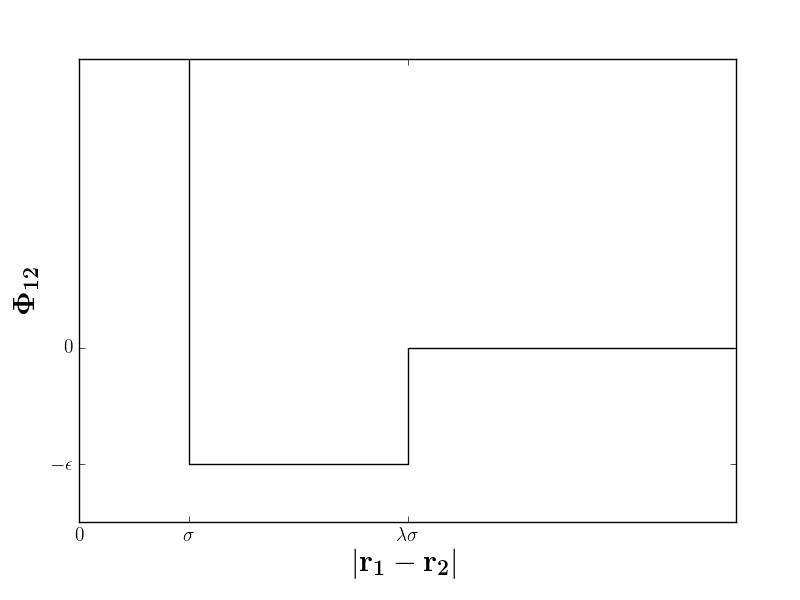
\includegraphics[width=.75\textwidth]{SWF-E.png}
    \caption{Demonstration of Square-Well approximation.}
    \label{sw_phi}
\end{figure}

\subsection{Critical Point} 
The critical point is the temperature and pressure (or any other thermodynamic pairing) on a phase diagram (shown in Figure ~\ref{phase}) where the line between liquid and vapor terminates - liquid and vapor become indistinguishable and are assimilated into the ``supercritical fluid'' phase. Many interesting effects occur here, including the well-researched phenomena of critical opalescence. The correlation length, loosely interpreted here as the maximum wavelength of the density fluctuations within the fluid, diverges to infinity near criticality. As mentioned previously, the diverging of the correlation length invalidates SAFT and many of its variants which assume constant density beyond small length scales. 
\begin{figure}
    \centering
    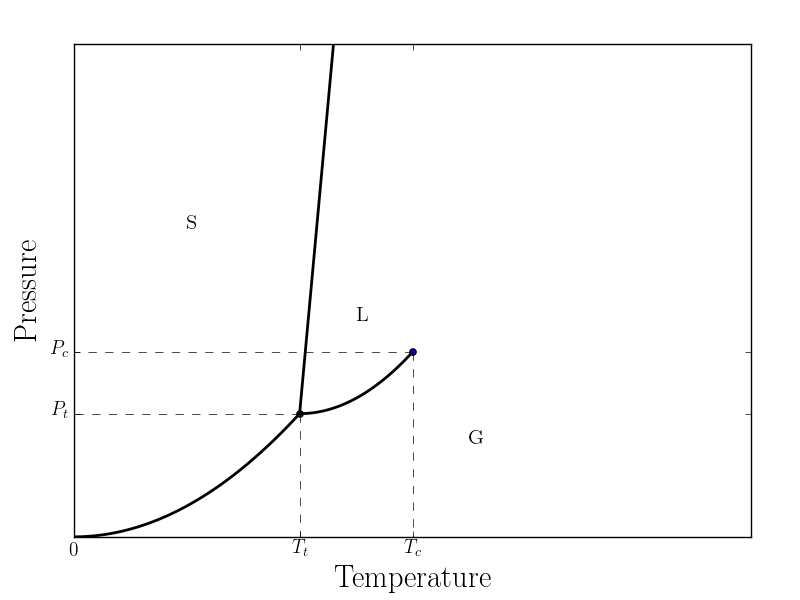
\includegraphics[width=.75\textwidth]{phase.png}
    \caption{Phase diagram of a liquid with critical point and triple point identified.}
    \label{phase}
\end{figure}
\\
The theory of this project is largely predicated upon the behavior of critical systems, namely the phenomena of self-similarity. Non-critical systems exhibit different characteristics when viewed at different length scales. Ever-present small-scale correlations (that is, fluctuations in density) are relevant, if not dominant, when viewing the system at very small scales, but typically become less important at larger scales and nearly irrelevant near the thermodynamic limit. Near the critical point all correlation wavelengths are present, and so the system looks the same regardless of length scale chosen. This self-similarity allows for the decomposition of the large critical cell to smaller constituent cells. The details of the procedure are more thoroughly discussed in Chapter.

\subsection{Free energy}
The energy we are interested in calculating is the ``absolute'' Helmholtz free energy $F^{\text{abs}}$. The Helmholtz free energy is a Legendre transform of the internal energy $U$
\begin{align}
    F &= U - TS\, ,
    \label{Fdef}
\end{align}
and can be calculated given the ever-pervasive partition function $Z$:
\begin{align}
    F &= -T \ln Z\, .
    \label{FdefSM}
\end{align}
With $F$ calculated, its partial derivatives yield all other interesting thermodynamic quantities. Though the Gibbs free energy yields the same information, the Helmholtz free energy is particularly useful because of the relationship with entropy, namely
\begin{align}
    S &= \left(\frac{\partial F}{\partial T}\right)_{V}\, .
\end{align}
Entropy is a very similar partial derivative of the Gibbs free energy, but with pressure held fixed instead of volume. We typically will want to hold volume fixed, so the Helmholtz free energy is the natural choice. Further, if we allow the number of particles in the system to vary, we will use the grand free energy $\Phi$, defined as
\begin{align}
    \Phi &= U-TS-\mu N\\
    &= F - \mu N
    \label{Phidef}
\end{align}
where $\mu$ is the chemical potential of the fluid, which is related to the tendency of particles to flow into or out of the system.\\

Equations~\ref{Fdef} and~\ref{FdefSM} together bridge classical thermodynamics and statistical mechanics. Due to the nature of this project, we will primarily be concerned with the statistical mechanics definition (that is, Eq.~\ref{FdefSM}) of the free energy. We are, then, ultimately concerned with determining the partition function for any given system. The canonical ensemble partition function can be compactly represented by a summation:
\begin{align}
    Z &= \sum^{\text{states}}~e^{-\beta E_i}
\end{align}
where $\beta =  T^{-1}$ and $E_i$ is the energy of the $i^{\text{th}}$ state. Of course, it is impractical to sum over the individual states of the system because the number of states of a classical system are generally innumerable. Instead we sum over energies:
\begin{align}
    Z &= \sum^{\text{energies}}~D(E)~e^{-\beta E_i}
\end{align}
where we have now introduced the density of states $D(E)$ which is a simple function that returns the number of states which have a given energy $E$. The density of states is now the focus of calculation - if we can accurately determine the density of states of the system, we can calculate the Helmholtz free energy and, from there, any other thermodynamic quantity we wish. \\  

Since $F$ contains a natural log term, we can separate and characterize the individual contributions of kinetic energy (``ideal'') and energy associated with the configuration of the system (``excess'').  
A derivation of the two energy contributions for a monoatomic fluid follows. \\

\ignore{{\color{red} [This should probably go in an appendix. Further: replace $Z_C$ with $Z_{exc}$; fix the to the N on the $Z_{exc}$ term; include the $N!$ into the ideal term; fix the $V(r_1, r_2, ...)$||| All done! NOW: fix the dimensions on the $Z_{id}$ term!]}}

We begin with the canonical form of the canonical ensemble partition function $Z$:
\begin{align}
    Z &= \sum_E D(E) e^{-\beta E}
\end{align}
where we sum over individual energies of the system $E_i$. However, to provide a general expression, we will instead sum over the states $s$:
\begin{align}
    Z &= \sum_s e^{-\beta E_s}
\end{align} 

Further, the energy of each state is simply the sum of the excess and kinetic energies $V$ and $K$, so

\begin{align}
    E_s &= V_s(\mathbf{r}) + K_s(\mathbf{p})
\end{align}

So now we have 

\begin{align}
    Z &= \sum_S e^{-\beta (V_s(\mathbf{r}) + K_s(\mathbf{p}))}\\
    &= \sum_S e^{-\beta V(\mathbf{r})}~e^{-\beta K(\mathbf{p})}
\end{align} 

Each state is specified by a particular point in phase space (parameterized by $\mathbf{r}$ and $\mathbf{p}$). Even though quantum mechanically this phase space is discrete, we can approximate the space as continuous by recognizing that the spacing between individual states is small compared to the total range of the states, so that the summation becomes an integral:

\begin{align}
    Z &= \int_s~ \diff\mathbf{r}~ \diff\mathbf{p} ~e^{-\beta V(\mathbf{r})}~e^{-\beta K(\mathbf{p})}
    %&= \sum_s e^{\beta V(\mathbf{r})}e^{-\beta T(\mathbf{p})}
\end{align} 
However, the above is only partially correct, as it is only for one particle. We can account for multiple particles by requiring that each particle has the same partition function contribution for kinetic energy; however, the potential energy does not separate as nicely since it depends on the position of all particles. For the kinetic energy, we are simply integrating $N$ times for $N$ particles:

\begin{align}
    Z &= \int_{s_1} \int_{s_2} \dots \int_{s_N} \diff\mathbf{r_1}~ \diff\mathbf{p_1} ~\diff\mathbf{r_2} ~\diff\mathbf{p_2} ~\dots ~\diff\mathbf{r_N}~ \diff\mathbf{p_N} ~e^{-\beta V(\mathbf{r_1}, \mathbf{r_2}, \dots \mathbf{r_N})}~e^{-\beta(K(\mathbf{p_1}) + K(\mathbf{p_2}) ... K(\mathbf{p_N}))}\\
    &= \int_s \diff\mathbf{r}^N ~e^{-\beta V(\mathbf{r_1}, \mathbf{r_2}, \dots \mathbf{r_N})} \left[\int_s \diff\mathbf{p}~e^{-\beta K(\mathbf{p})}\right]^{N}
    \label{Z-intermed}
\end{align}
where we have separated the integrals by recognizing that the integrands are independent.\\
Additionally, for a proper quantum mechanical treatment we must assume that the particles are indistinguishable which means the above expression over-counts by a factor of $N!$. Additionally, we will multiply Eq. \ref{Z-intermed} by an overall factor of $\frac{V^N}{V^N}$ to preserve units and extensivity. Our expression for the partition function is then 

\begin{align}
    Z &= \frac{1}{ N!}\int_s \frac{\diff\mathbf{r}^N}{V^N} ~e^{-\beta V(\mathbf{r_1}, \mathbf{r_2}, \dots \mathbf{r_N})} \left[\int_s V\,\diff\mathbf{p}~e^{-\beta K(\mathbf{p})}\right]^{N}
    \label{Z_full}
\end{align}

We then define the two factors obvious in Eq. \ref{Z_full}, the excess factor dependent on the potential energy $V(\mathbf{r})$ and the ideal factor dependent on the kinetic energy $K(\mathbf{p})$: 

\begin{align}
    Z &= (Z_{exc})(Z_{id}) \,,
\end{align}
where $Z_{id}$ contains the $N!$ term by convention. The excess term $Z_{exc}$ is system dependent because $V(\mathbf{r})$ is buried inside the integral, but the ideal factor is the same for any system where the total energy separates in the preceding fashion. We judiciously decide to leave the excess factor alone, for now, and work specifically with the ideal term. We then have

\begin{align}
    Z_{id} &=  \frac{1}{N!}\left[\int_s \diff\mathbf{p} ~e^{-\beta K(\mathbf{p})}\right]^{N}
\end{align}

We begin by imagining a cell of length $L$ and volume $L^3$ in which lives a particle. Then, we quantize the allowed wavelengths of the particle within the cell by defining the wavevector $\mathbf{k}$ as
\begin{align}
    \mathbf{k} &= \frac{2\pi}{L}(n_x\mathbf{\hat{x}} + n_y\mathbf{\hat{y}} + n_z\mathbf{\hat{z}})
\end{align}
Remembering that kinetic energy can be expressed as $K = \frac{\hbar^2 k^2}{2m}$, and using our definition of $\mathbf{k}$:
\begin{align}
    Z_{id} &= \frac{1}{N!}\left[\int_s V\, \diff\mathbf{p} ~e^{-\beta \frac{\hbar^2 k^2}{2m}}\right]^{N}
    \label{Zt_def}
\end{align}
This unfortunately introduces a mass quantity into the partition function which adds an additional parameter that needs to be determined to properly account for quantum mechanical effects. If we then allow the cell to become very large, then the we can easily see in Eq. \ref{Zt_def} that the spacing between occupants in phase space becomes small, so we can integrate instead $\diff ^3 n$ over all possible values of $n$:
\begin{align}
    Z_{id} &= \frac{1}{N!}\left[\int_0^\infty \diff^3 n ~e^{-\frac{\beta \hbar^2}{2m} \left(\frac{2\pi}{L}(n_x\mathbf{\hat{x}} + n_y\mathbf{\hat{y}} + n_z\mathbf{\hat{z}}\right)^2}\right]^{N} \\
    &= \frac{1}{N!}\left[\int_0^\infty \diff^3 n ~e^{ \frac{-2\beta \hbar^2\pi^2}{mL^2}(n_x^2 + n_y^2 + n_z^2)}\right]^{N}
\end{align}
where extra factors of $\hbar $and$ \pi$ were gained from the change of variables. Evaluating this integral yields
\begin{align}
    Z_{id} &= \left(\frac{V^N}{N!\Lambda^{3N}}\right) \,, \\
    \Lambda &= \frac{\hbar\sqrt{2\pi}}{\sqrt{mT}}
\end{align}
where we have introduced the thermal deBroglie wavelength $\Lambda$ which defines the de Broglie wavelength of an ideal gas at a temperature $T$. The full partition function for any monoatomic system is then
\begin{align}
    Z &= Z_{exc} \left(\frac{V}{N!\Lambda^{3}}\right)^{N} \,.
\end{align}
For liquids, the $Z_{exc}$ factor is difficult to evaluate; the hard sphere liquid, the simplest model for a dense fluid, does not have an analytic representation for the excess free energy. It follows that a considerable amount of work is required to determine the excess free energy for a given system. The absolute free energy, by way of Eq. \ref{FdefSM}, now has the form
\begin{align}
    F_{abs} &= -T\,\ln\left(Z_{exc} \frac{V^N}{N!\Lambda^{3N}}\right)\\
    &= -T\ln\left(Z_{exc}\right)\, -T\ln\left(\frac{V}{(N!)^{1/N}\Lambda^3} \right)^N\\
    &= -T\ln\left(Z_{exc}\right) - NT\ln\left(\frac{V}{\Lambda^3}\right) + NT\ln\left(N!^{1/N}\right)\\ 
\end{align}
Redefining the first factor including $Z_{exc}$ to be $F_{exc}$, and then using Sterling's approximation ($\ln(N!) = N\ln N - N$ for large N), we arrive at \textcolor{red}{BRENDEN FIX: $N\ln N - N$, plus I think we may want to add to the excess free energy (probably to the excess HS entropy?) the difference?}
\begin{align}
    F_{abs} &= F_{exc} - NT\left(\ln\left(\frac{V}{\Lambda^3}\right) - \ln\left(N\right) + 1\right)
\end{align}
At a specified volume and number of particles, the ideal gas contribution is only a function of temperature. Consequently, for a given temperature we only need to compute the excess free energy.
%%%%%%%%%%%%%%%%%%%%%%%%%%%%%%%%%%%%%%%%%%%%%%%%%%%%%%%%%%%%%%%%%%%%%%%
%                            METHODS                                  %
%%%%%%%%%%%%%%%%%%%%%%%%%%%%%%%%%%%%%%%%%%%%%%%%%%%%%%%%%%%%%%%%%%%%%%%

\section{Methods}
This work requires the intersection of three methods to calculate the absolute free energy $F_{abs}$ of the bulk cell. A preliminary value of the free energy of the bulk can be obtained from Monte Carlo simulations. This value can then be made absolute by carefully comparing the results with thermodynamic integration, a method of determining the free energy of the hard-sphere system. The resulting absolute free energies for each fluctuation length can be summed to yield the absolute free energy of the bulk. {\color{red}[deal with the problems here]} 

\subsection{Monte Carlo Methods}

Unbiased Monte Carlo methods utilize random or pseudorandom sampling and check for certain conditions or measure certain quantities after a specified number of iterations. Traditional random sampling requires that the current step, or ``move'', is irrespective of previous steps. True random movement is an ideal simulation characteristic for the canonical ``drunken rambler'' scenario, in which a intoxicated man attempts to make his way home by taking random steps. Since the drunken man chooses his next move arbitrarily, his movement is considered ``random''; it follows that true random sampling is desirable for this physical system. \\

Statistical mechanics, however, does not exhibit this independence. Each time the drunken man makes a move there is an equal probability that he will move in any particular direction. Rather than all movements having equal probability, statistical mechanics stipulates that the probability of a particular move occurring depends explicitly upon the energy difference of the current and resulting configurations. Instead of true random Monte Carlo methods, we clearly need some way to control the probability of transitions from a given state. In pursuit of this control, we employ the method of Markov chains, specifically broad histogram transition matrix Monte Carlo.
\subsubsection{Metropolis-Hastings}
Metropolis-Hastings Monte Carlo methods eschew the true randomness of unbiased Monte Carlo by taking the current configuration into account before moving. If we define the ensemble of states of the system in equilibrium by a vector column $\mathbf{q}$, and the resulting state $\mathbf{p}$ after a single time step, the relationship
\begin{align*}
    \mathbf{p} &= \mathcal{P}\, \mathbf{q}\\
\end{align*}
defines a ``transition'' of the system. $\mathcal{P}$ is a necessarily square matrix that contains information about these transitions. We call this construction $\mathcal{P}$ the {\it transition matrix}. This matrix is $L\times L$, where $L$ is the number of energy levels in system. If all rows of the transition matrix are , we can see that any state of the system is reachable after a finite number of transitions from any given initial state. A physically correct simulation will generate a transition matrix that satisfies the thermodynamic steady state condition; given the ensemble of equilibrium states $\mathbf{q}_{eq}$, we enforce that
\begin{align}
    \mathcal{P}\,\mathbf{q}_{eq} &= \mathbf{q}_{eq}
    \label{thermo-steady-state}
\end{align}
The transition matrix thus embodies the physics of the simulation.

\subsection{Broad Histogram Monte Carlo}
If the energy of the system at each time step in a Monte Carlo simulation is recorded, it is straightforward to construct a histogram of energies. That is, a histogram with a bin for each narrow $\Delta E$ around a value $E$ that counts the number of times the system visited that energy range. Typical implementations of histogram methods follow the ``canonical histogram'' procedure outlined by Ferrenberg and Swendsen \cite{ferrenberg1988histogram} -- given a histogram $h_T(E)$ extracted from a simulation at some temperature $T_0$, a reweighting scheme can then extend the histogram to any other temperature $T$ via 
\begin{align}
    h_{T}(E) &= h_{T_0}(E) \exp\left(E/T - E/T_0 \right)
\end{align}
and then normalizing appropriately. This method unfortunately loses substantial accuracy far from the original temperature and causes an untoward spike near the average value of the original histogram. Further, this reweighting detracts from the accuracy of the tails of the histogram. We choose instead to implement a similar approach to that of de Oleveira and coworkers\cite{de1998broad}, the ``broad histogram''. \\

To construct the broad histogram we need to perform a Markovian walk along the energy levels of the system. Throughout the walk we count the number of times we transitioned from a given initial energy to to a given resulting energy. If we walk across the entire energy range, we can construct histogram of energy transitions $h(E_i, E_j)$ for all $i, j$. The walk goes as follows: starting with a state $\mathbf{q_i}$ with energy $E_i$, we attempt perform a random move to a state $\mathbf{q_f}$ with energy $E_f$. Assuming the resulting configuration is valid, the move is always accepted if the energy decreases, i.e, $E_f - E_i <0$. Otherwise, we accept the move with a probability related to the ratio of counts of the transition occurring ``forwards'' to the transition occurring the opposite direction. Since each state is reachable within a finite amount of time in a Markovian process, a broader, more accurate histogram merely requires more computation time. This process is outlined in Algorithm~\ref{alg_tmmc}.\\

\begin{algorithm}[tb]
    \caption{Transition Matrix Monte Carlo Initialization}
    \label{alg_tmmc}
    \hrulefill
    \begin{enumerate}
        \item Begin state $\mathbf{q_0}$ and a zero transition matrix.
        \item Perform a random walk, transitioning from an initial state $\mathbf{q_i}$ to a final state $\mathbf{q_{f}}$. Initially accept the state if the configuration is valid. \label{alg-tmmc-start}
        \item Increment the transition histogram $h(E_i, E_f)$.
        \item Accept move unconditionally if $\Delta E_f - E_i = E < 0$.
        \item Else, accept move with a probability proportional to $\frac{h(E_i, E_f )}{h(E_f, E_i)}$.
        \item If not end condition has been met, return to step \ref{alg-tmmc-start}.   
    \end{enumerate}
    \hrulefill
\end{algorithm}

Calculating the density of states, given the transition matrix constructed via the process in Algorithm~\ref{alg_tmmc}, is a trivial matter. The equilibrium condition given in Eq.~\ref{thermo-steady-state} is really a statement about the density of states; for a Monte Carlo simulation, the equilibrium state $q_{eq}$ is exactly the density of states. Solving the steady state condition as an eigenvalue problem for $q_{eq}$ then yields the density of states\cite{perlinthesis}. \\

It bears mentioning that most implementations of transition matrix methods consider the above procedure the ``initialization'' process. The canonical ``simulation'' period refers to gathering statistics for quantities that cannot be calculated from the density of states, such as the density of the fluid or the pair distribution function. Given that we only are concerned with quantities that can be computed given the density of states, we never actually ``simulate''. With the density of states computed, we can now calculate the partition function and thereby the free energy.

\subsection{Renormalization Group Theory}
Renormalization group methods attempt to describe how a particular system's properties are altered when the system is viewed from varying length scales. Near the critical point, the fluid becomes self similar, and so fluctuations of all wavelengths are present. We can then compare quantities of related yet physically different systems as they all exhibit the similar properties.\\
We begin with a periodic cubic cell of length $L_0$ and volume $L_0^3$. 
This cell has periodic boundary conditions and consequently allows for fluctuations up to wavelength $L_0$. These fluctuations contribute some absolute free energy $F_0$ to the absolute free energy of the full cell. We then double the length of the cell to allow for fluctuations of up to wavelength $L_0$. We continue this process until all relevant wavelengths have been included. Adding up the change in absolute free energy calculated in this manner then yields the total free energy of the critical system, which can then be compared to accepted simulation methods. Algorithm~\ref{alg_renorm} details this process. 

\begin{algorithm}[tb]
    \caption{Renormalization-esque calculation of total free energy}
    \label{alg_renorm}
    \hrulefill
    \begin{enumerate}
        \item Simulate smallest cell of length $L_0$.
        \item Calculate absolute free energy from simulation output.
        \item Simulate new cell with same density but octupled volume of previous cell.
        \item Calculate absolute free energy from simulation output.
        \item Calculate change in absolute free energy between the current regime and the last, add to running $\Delta F^{\text{abs}}_{\text{tot}}$
        \item Repeat 3-4 for each desired doubling regime.
    \end{enumerate}
    \hrulefill
\end{algorithm}

Eq. ~\ref{GRGT-F1} details the mathematics of this coupling procedure.

\begin{align}
    \label{GRGT-F1}
    F^{\text{abs}}_{\text{tot}} = \sum_{i=1}^{k}\Delta F^{\text{abs}} &= \lim_{k\to\infty}\sum_{i=1}^{k} F^{\text{abs}}_{i} - F^{\text{abs}}_{i-1}\\
    &\approx \sum_{i=1}^{k} F^{\text{abs}}_{i} - F^{\text{abs}}_{i-1}
    \label{GRGT-F2}
\end{align}

Strictly speaking, a formal limit is required for equality in Eq.~\ref{GRGT-F1}, rather than only including wavelengths up to $2^k\lambda_0$. Though theoretically all wavelengths are present at the critical point it is only necessary to include the first several to accurately describe systems moderately close to the critical point. Given approximation, we choose instead to use Eq.~\ref{GRGT-F2}. Each $F^{\text{abs}}_i$ can be calculated using a combination of different Monte Carlo methods, namely Metropolis-Hastings Monte Carlo and thermodynamic integration. A graphical representation of this process can be shown in Figure ~\ref{GRTG-demo}.\\

%%%%%%% TIKZZZZZ%%%%%%%



\begin{figure}
\centering
    \resizebox{.75\textwidth}{!}{
     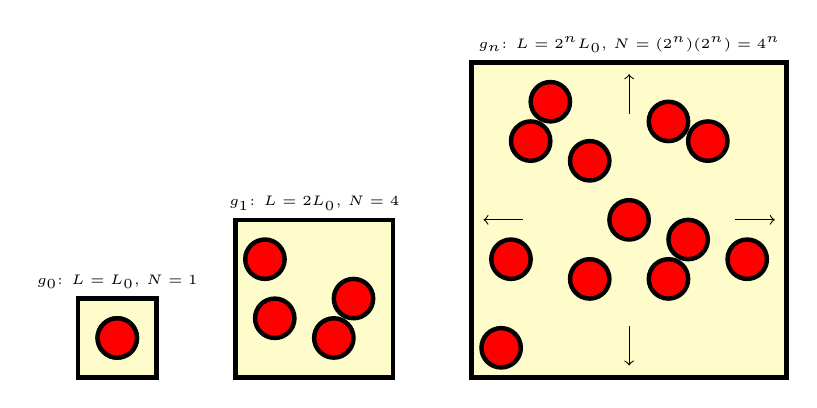
\begin{tikzpicture}
            \draw[black, ultra thick, fill=yellow, fill opacity=.2] (0,0) rectangle (1,1);
            \draw[black, ultra thick, fill=yellow, fill opacity=.2] (2,0) rectangle (4,2);
            \draw[black, ultra thick, fill=yellow, fill opacity=.2] (5,0) rectangle (9,4);
            %\draw[black, ultra thick, fill=yellow, fill opacity=.2] (10,0) rectangle (14,4);
            \draw[<-] (5.15,2) to (5.65,2);
            \draw[->] (7,3.35) to (7,3.85);
            \draw[<-] (7,.15) to (7,.65);
            \draw[->] (8.35,2) to (8.85,2);
            \node[above] at (.5,1) {\tiny $g_0$: $L=L_0$, $N=1$};
            \node[above] at (3,2) {\tiny $g_1$: $L=2L_0$, $N=4$};
            %\node[above] at (7,4) {\tiny $g_2$: $L=4L_0$, $N=8$};
            \node[above] at (7,4) {\tiny $g_n$: $L=2^nL_0$, $N=(2^n)(2^n)=4^n$};

            % Balls!
            \draw[ultra thick, fill=red] (.5,.5) circle [radius=.25];
            % Second box
            \draw[ultra thick, fill=red] (3.25,.5) circle [radius=.25];
            \draw[ultra thick, fill=red] (3.5,1) circle [radius=.25];
            \draw[ultra thick, fill=red] (2.375,1.5) circle [radius=.25];
            \draw[ultra thick, fill=red] (2.5,.75) circle [radius=.25];
            % third
            \draw[ultra thick, fill=red] (5.5,1.5) circle [radius=.25];
            \draw[ultra thick, fill=red] (5.375,.375) circle [radius=.25];
            \draw[ultra thick, fill=red] (6,3.5) circle [radius=.25];
            \draw[ultra thick, fill=red] (7.5,3.25) circle [radius=.25];
            \draw[ultra thick, fill=red] (.5,.5) circle [radius=.25];    
            \draw[ultra thick, fill=red] (7,2) circle [radius=.25];        
            \draw[ultra thick, fill=red] (5.75,3) circle [radius=.25];        
            \draw[ultra thick, fill=red] (6.5,2.75) circle [radius=.25];        
            \draw[ultra thick, fill=red] (8, 3) circle [radius=.25];        
            \draw[ultra thick, fill=red] (7.5,1.25) circle [radius=.25];        
            \draw[ultra thick, fill=red] (7.75,1.75) circle [radius=.25];        
            \draw[ultra thick, fill=red] (8.5,1.5) circle [radius=.25];
            \draw[ultra thick, fill=red] (6.5,1.25) circle [radius=.25];                
     \end{tikzpicture}}
\caption{2-D Demonstration of MC-GRGT doubling method.}
\label{GRTG-demo} 
\end{figure} 


%%%%%% TIKZZZZ %%%%%%


\subsection{Thermodynamic Integration}
\subsubsection{General Process}
Thermodynamic integration is a unique way to determine the ``excess'' free energy of the system. Using hard sphere Monte Carlo, we transition from a filling fraction of zero to a dense system with filling fraction $\eta_{max}$, calculating the change in free energy at each step. When we have reached the desired final filling fraction we have found the free energy that was necessary to create that configuration of particles - this is exactly the absolute free energy of the system.\\
\subsubsection{Algorithm}
The hard sphere fluid is simple to work with since its partition function simply counts the number of microstates in the system\cite{valeskethesis}. Since we are calculating the change in free energy as we transition to higher and higher filling fractions, we need only be concerned with finding the ratio of partition functions between each step. Since the hard sphere partition function is a ``counting'' mechanism, we can determine this ratio using Monte Carlo simulations. Given a starting state (defined by the arrangement of particles and filling fraction) we shrink the volume and intermolecular distances by a scaling factor and then see if the resulting configuration of particles is valid. If the configuration is valid, we accept it as also valid in the small cell and then return to the original configuration. If the resulting configuration is invalid, we count the move as failed. This process continues until a predefined number of iterations are completed.\\


Once a count of valid and failed moves for a given filling fraction step has been established, the entropy of the system can be determined. Give $N_i$ total checks of the small cell during the $i^{\text{th}}$ step, $M_i$ of which were valid, the entropy calculated integrating from a filling fraction of $\eta=0$ to some $\eta_f$ in $K$ steps is
\begin{align}
    S_{HS,~exc} &= \sum_i^K \ln\left(\frac{M_i}{N_i-M_i}\right)
\end{align}

\begin{algorithm}[!b]
\caption{Thermodynamic integration.}
\label{alg:ti}
\begin{alg}
\item Construct cell with desired number of spheres with filling fraction of zero.
\item Move spheres random fractions of a predefined translation distance. \label{alg-ti-move}
\item Repeat step \ref{alg-ti-move} for desired number of iterations before checking the small cell.
\item Check the ``small cell'' by shrinking the volume and determine whether or not the configuration is still valid.
\item If configuration is still valid, increment the count of valid checks.
\item If configuration is invalid, increment the count of failed checks. \label{alg-ti-move-end}
\item Repeat steps \ref{alg-ti-move} - \ref{alg-ti-move-end} until desired iterations reached.

\end{alg}      
\end{algorithm}  


%TIKZ
\begin{figure} \centering
    \resizebox{.75\textwidth}{!}{
    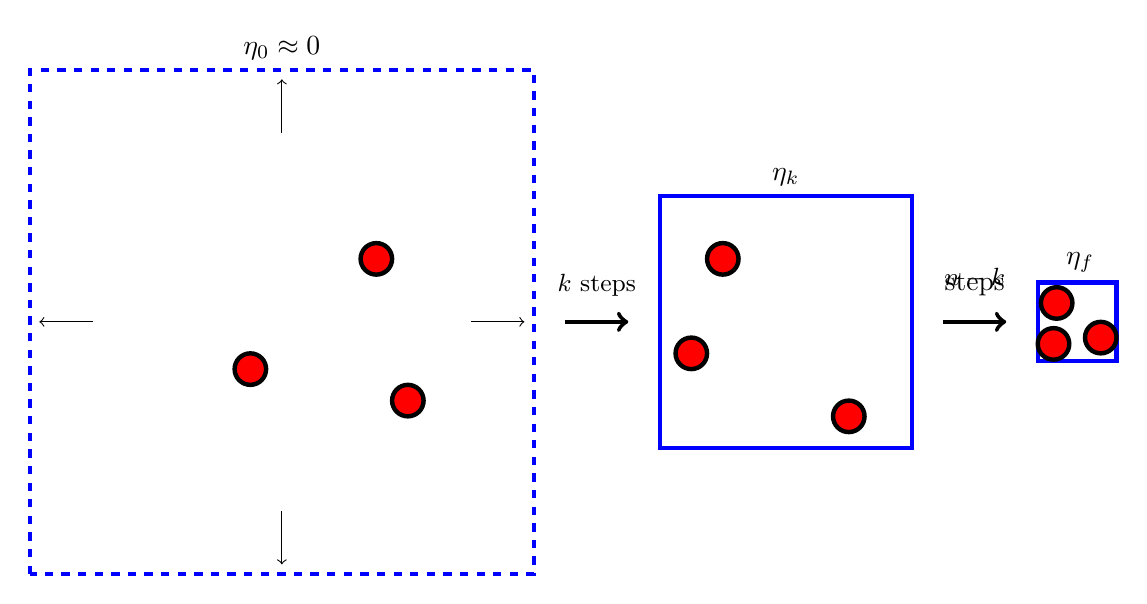
\begin{tikzpicture}[scale=.8,  auto]
    \draw[blue, ultra thick] (10,3) rectangle (14,7);
    \draw[blue, ultra thick, dashed] (0,1) rectangle (8,9);
    \draw[blue, ultra thick] (16,4.375) rectangle (17.25,5.625);
    \draw[->] (4,8) to (4, 8.85);
    \draw[->] (7,5) to (7.85, 5);
    \draw[->] (1,5) to (.15, 5);
    \draw[->] (4,2) to (4, 1.15);
    \draw[ultra thick, ->] (8.5,5) to (9.5,5);  
    \node [above] at (9,5.25) {\small $k$ steps};
    \draw[ultra thick, ->] (14.5,5) to (15.5,5);
    \node[align=center] [above] at (15, 5.25) {\small $n-k$ \\[-1em] steps};
    \draw[ultra thick, fill=red] (3.5,4.25) circle [radius=.25];
    \draw[ultra thick, fill=red] (6,3.75) circle [radius=.25];
    \draw[ultra thick, fill=red] (5.5,6) circle [radius=.25];
    \draw[ultra thick, fill=red] (10.5,4.5) circle [radius=.25];
    \draw[ultra thick, fill=red] (13,3.5) circle [radius=.25];
    \draw[ultra thick, fill=red] (11,6) circle [radius=.25];
    \draw[ultra thick, fill=red] (16.3,5.3) circle [radius=.25];
    \draw[ultra thick, fill=red] (17,4.75) circle [radius=.25];
    \draw[ultra thick, fill=red] (16.25,4.65) circle [radius=.25];
    \node [above] at
     (4,9) {$\eta_0 \approx 0$};
    \node [above] at (12,7) {$\eta_k$};
    \node [above] at (16.675,5.625) {$\eta_f$}; 
    \end{tikzpicture}}
    \caption{Demonstration of filling fraction increase during thermodynamic integration from $\eta=0$ to $\eta=\eta_f=\eta_{max}$.}
    \label{TI-demo}
\end{figure}



Combining Eq.~\ref{C-S-eq} with a simple bisection method allows for control of the filling fraction step size given a desired change in free energy. We determined that steps yielding an approximate change in specific absolute free energy of $\Delta F^{abs}/NT = \ln(2)$ through trial and error - smaller step sizes unnecessarily increased simulation time and larger step sizes tended to shrink too quickly causing the simulation to miss relevant states in the system. This step size corresponds to changing the entropy by $1/2$ each step. 

\ignore{NB: is there a more physical reason we chose this filling fraction increase?}

\subsection{Data Storage}
All simulation output is saved in text files for plotting and visualization ease. The question of organization becomes important with this amount of files being generated. Each different system simulation (length $L = \sqrt2 \sigma, 5,10$) has data regarding each doubling regime ($i=0,1,2,3?$) and each doubling regime contains data for each possible sphere count ($N=1,2,3\dots N_{max}$, where $N_{max}$ is typically limited by maximal sphere packing of $N_{max}/L^3\approx.741$). The file structure mirrors the above symmetry: 
\begin{align*}
                &\rightarrow \text{i=0} &\rightarrow \text{N=0}\\
                & &\rightarrow \text{N=1}\\
                && \vdots\\
\text{System} & \rightarrow \text{i=1} &\rightarrow \text{N=0}\\
                && \rightarrow \text{N=1}\\
                &&\vdots\\
                &\rightarrow \text{i=2} &\rightarrow \text{N=0}\\
                && \rightarrow \text{N=1}\\
                &&\vdots\\
\end{align*}
Each sphere count subfolder contains a single text file from TMMC output and another subfolder where all of the thermodynamic integration output is stored. Each thermodynamic integration simulation outputs a single text file upon completion of each filling fraction step. On average, a single calculation requires approximately $175$ steps. This structure was chosen both for elegant parallelism and for plotting accessibility. 

\subsection{Calculating the Absolute Free Energy}
{\color{red} please rewrite me. This paragraph has been terrible since it was written.}\\
It is straightforward the compute a Helmholtz free energy through the Monte Carlo simulations; the difficulty in this method lies in computing the correct free energy. TMMC, as mentioned previously, yields a free energy accurate only up to a unknown constant. Since we need to add up changes in free energy across multiple simulations, we need each calculated free energy to be ``absolute'' - that is, we must eliminate this unknown constant. \\

At infinite temperature, the square well fluid has approximately the same behavior as the hard sphere fluid.  We assert that the correct inclusion, then, is to enforce that the excess entropy calculated via TMMC at $T=\infty$ is equal to the hard sphere entropy calculated through thermodynamic integration. We do this by exploiting the infinite temperature behavior of the canonical ensemble:
\begin{align}
    Z_{\infty} &= \left.\sum_{i=0}^{\text{\tiny Energies}} D(E) e^{-\beta E}\right|_{\beta = 0}\\
    &= \sum_{i=0}^{\text{\tiny Energies}} D(E)\\
    &= \#\text{~states}\;.
\end{align}

The partition function now calculates the total number of states in the system which we expected due to the equipartition theorem. The excess free energy is simply
\begin{align}
    F_{SW,~exc} &= U_{SW,~exc} - T\,S_{SW,~exc}     
\end{align} 
and, at infinite temperature, the internal energy asymptotes to a value independent of temperature, leaving us with
\begin{align}
    F_{SW,~exc} &= -T\,S_{SW, ~exc} + U_{exc}\;.
\end{align}

The hard sphere system has no excess internal energy, so the excess free energy is merely
\begin{align}
     F_{HS,~exc} &= -T\,S_{HS,~exc} 
\end{align} 

Since the excess hard sphere free energy is really just the entropy \cite{valeskethesis} (scaled by temperature), the statement that the square well and hard sphere excess free energies need be equal in the infinite temperature limit is really a constraint on the {\it entropy} of the two systems. We then conclude that
\begin{align}
    S_{SW,~exc} \Bigm\lvert_{T=\infty} &= S_{HS,~exc}
\end{align}

\subsection{Thermodynamic Quantities from Simulation}
Given the density of states output $\ln[D(E)]$ from the Monte Carlo simulation, combined with {\it a priori} knowledge that the system obeys a canonical ensemble distribution of states, we can calculate any thermodynamic , for instance, the excess internal energy:
\begin{align}
     U_{exc}(T) &= \frac{\sum_{i=0}^{\text{\tiny Energies}}\,E_i\, \exp(\ln[D(E)] - \beta E_i)}{\sum_{i=0}^{\text{\tiny Energies}} \exp(\ln[D(E)] - \beta E_i)}\\
     &= \frac{\sum_{i=0}^{\text{\tiny Energies}} E_i \exp\left(-\beta E_i\right)}{Z}
\end{align} 
where, as usual, $\beta = T^{-1}$.  unfortunately, tends to introduce overflow or underflow errors during computation. We combat this by subtracting the maximum value of the natural log of the density of states \ignore{subtracting maximum ought to make it more negative\dots}from each element of $D(E)$, and then adding the maximum back in after the exponential. We calculate the excess free energy by using the entropy equality developed previously:
\begin{align}
     S_{SW,~exc}\Bigm\lvert_{T=\infty} &= S_{HS,~exc}\\
     \implies F_{SW,~exc}\Bigm\lvert_{T=\infty} &= U_{SW,~exc}\Bigm\lvert_{T=\infty} -TS_{HS,~exc} \\
     \implies F_{SW,~exc}(T) &= F_{SW,~exc}\Bigm\lvert_{T=\infty} + \left(F_{SW,~exc}(T) - F_{SW,~exc}\Bigm\lvert_{T=\infty}\right)
     \\
     \implies F_{SW,~exc}(T) &= U_{SW,~exc}\Bigm\lvert_{T=\infty} -TS_{HS,~exc} + \left(F_{SW,~exc}(T) - F_{SW,~exc}\Bigm\lvert_{T=\infty}\right)
     \\
     F_{SW,~exc} &= U_{\infty} -TS_{HS,~exc} - T\ln\left(\frac{Z}{Z_{\infty}}\right)
\end{align} 
The excess hard sphere entropy $T_{HS,~exc}$ is calculated directly from thermodynamic integration, $Z$ is calculated using  . Once we have calculated both the excess free energy and excess internal energy, we can directly find the excess entropy:
\begin{align}
    S_{SW, ~exc} &= \frac{1}{T}\left(U_{SW,~exc} - F_{SW,~exc} \right)
\end{align}


\section{Results}
An important remaining question is whether there is a preferred choice of minimum cell length. Physically we would [might?] expect that there is some dominant minimum fluctuation in the bulk cell - this would then lend a natural decision for the minimum cell length $\lambda_0$. Unfortunately we do not know this {\it a priori}, so we are reduced to guessing. Using the coupling procedure outlined previously, we calculated changes in free energy up to the $n^{\text{th}}$ doubling regime for several different cell lengths. We choose to focus on the ``scrunched'' case where the cell length is $\sqrt2\sigma$.\\

Figures ~\ref{F-T} through ~\ref{F-eta} show several computed thermodynamic quantities for the scrunched system. Each plot contains calculated quantities for either the first two doubling regimes or the first three. Calculations from the first doubling regime ($L=\lambda_0$) are solid lines, with the second doubling regime ($L = 2\lambda_0$) in dashes and the third ($L = 4\lambda_0$), when present, in circles . It is worth noting that the succeeding plots with respect to density have been interpolated; with a fixed cell size, it is only possible to simulate discrete filling fractions. The intervening points have been filled in using the Carnahan-Starling equation of state.\\  
\begin{figure}  
\centering
    \includegraphics[width=.75\textwidth]{../renormalization/figs/Fexc-vs-T.pdf}
    \caption{Excess specific free energy as a function of temperature.}
    \label{F-T}
\end{figure}

Figure \ref{F-T} shows expected behavior. As a function of temperature, the excess free energy monotonically increases for all densities tested. We see a positive free energy because $F = U -TS$; as temperature increases without bound, entropy remains negative and [blah blah more].\\

\begin{figure}
\centering
    \includegraphics[width=.75\textwidth]{../renormalization/figs/Shs-vs-eta.pdf}
    \caption{Excess hard sphere entropy as a function of density.}
    \label{Shs-eta}
\end{figure}
\ignore{Filling fraction or density? Value in distinction? We never use number density for the sake of units...}
Figure \ref{Shs-eta} shows the computed excess entropy as a function of density. We see that the both the first and second doubling regime closely match the Carnahan-Starling prediction for the entropy. After freezing, the first doubling regime veers from the prediction by the Carnahan-Starling equation of state; since the Carhan-Starling approximation is accurate only for low density fluids, we expect this behavior.\\

\begin{figure}
    \centering
    \includegraphics[width=.75\textwidth]{../renormalization/figs/Uexc-vs-eta.pdf}
    \caption{Excess internal energy as a function of density. The $x$ markers connected by dashed lines delineate second doubling regime densities that were simulated.}
    \label{U-eta}
\end{figure}
We see in Figure~\ref{U-eta} that the excess internal energy, as we would expect, becomes more negative as the density increases. The lower the temperature, the more ``clumped'' the system becomes, resulting in lower internal energies. [correct?]

\begin{figure}
\centering
    \includegraphics[width=.75\textwidth]{../renormalization/figs/Fexc-vs-eta.pdf}
    \caption{Excess specific free energy as a function of density.}
    \label{F-eta}
\end{figure}

\subsection{Primitive Cell}
The ``scrunched'' system allows exactly four spheres to be packed -- at maximal filling fraction $\eta_{max} = \approx .741$ -- in the original non-doubled cell. This case corresponds to the unit cell a face-centered cubic lattice, the simplest sphere packing possible. We chose to focus on the scrunched case for two reasons. Firstly, if any physical length of the system is likely to be the correct choice for minimum fluctuation length.

%%%%%%%%%%%%%%%%%%%%%%%%%%%%%%%%%%%%%%%%%%%%%%%%%%%%%%%%%%%%%%%
%                       Discussion                            %
%%%%%%%%%%%%%%%%%%%%%%%%%%%%%%%%%%%%%%%%%%%%%%%%%%%%%%%%%%%%%%%

\section{Discussion}
If the decomposition procedure outlined previously proves successful, the absolute free energy ought to obey known physics about the system.
We particularly care about identifying liquid-vapor coexistence within the fluid. \\

Finding coexistence requires use of the grand free energy $\Phi$. Liquid and vapor are simultaneously present in the fluid at densities that cause local minima in the grand free energy. We know that the grand free energy has a guaranteed minimum at the origin because [things]; we then only need to identify the other minimum.  \\

Referring back to Eq.~\ref{Phidef}, we can compute an absolute grand free energy given the absolute free energy and number of spheres. The chemical potential $\mu$ is a somewhat unintuitive quantity that, for our purposes, we will treat as a free parameter. Tweaking the value of the chemical potential will allow us to easily identify second minima in the grand free energy, and thereby the densities of the liquid and vapor present in the system.
\begin{figure}
\centering
    \includegraphics[width=.75\textwidth]{../renormalization/figs/Phiabs-vs-eta.pdf}
    \caption{Absolute grand free energy as a function of density.}
    \label{Phi-eta}
\end{figure}
Figure \ref{Phi-eta} 
%%%%%%%%%%%%%%%%%%%%%%%%%%%%%%%%%%%%%%%%%%%%%%%%%%%%%%%%%%%%%%%%%%
%                             CONCLUSION                         %
%%%%%%%%%%%%%%%%%%%%%%%%%%%%%%%%%%%%%%%%%%%%%%%%%%%%%%%%%%%%%%%%%%


\section{Conclusion}
We have presented a method by which the properties of bulk fluids can be estimated by decomposing the bulk into individual cells in a renormalization-minded manner by exploiting the critical behavior of fluids. The free energy contribution of each length scale can then be investigated and compared, both to determine the most energetic density fluctuations and to provide calculations that serve as a intermediate comparison with SAFT methods. This method is immediately applicable to any system where the energy of a configuration is straightforward to compute (that is, relatively inexpensive computationally). The application presented was a system that obeys the canonical ensemble, but the extension to the grand canonical ensemble can be done with little modification. Future work can include investing further doubling regimes ($i\geq 3$). 
%\bibliographystyle{plain}
\cleardoublepage
\bibliography{./Thesis}
\end{document}
